\documentclass[]{article}
\usepackage[T1]{fontenc}
\usepackage{lmodern}
\usepackage{amssymb,amsmath}
\usepackage{ifxetex,ifluatex}
\usepackage{fixltx2e} % provides \textsubscript
% Set line spacing
% use upquote if available, for straight quotes in verbatim environments
\IfFileExists{upquote.sty}{\usepackage{upquote}}{}
\ifnum 0\ifxetex 1\fi\ifluatex 1\fi=0 % if pdftex
  \usepackage[utf8]{inputenc}
\else % if luatex or xelatex
  \ifxetex
    \usepackage{mathspec}
    \usepackage{xltxtra,xunicode}
  \else
    \usepackage{fontspec}
  \fi
  \defaultfontfeatures{Mapping=tex-text,Scale=MatchLowercase}
  \newcommand{\euro}{€}
\fi
% use microtype if available
\IfFileExists{microtype.sty}{\usepackage{microtype}}{}
\usepackage[margin=1in]{geometry}
\usepackage{graphicx}
% Redefine \includegraphics so that, unless explicit options are
% given, the image width will not exceed the width of the page.
% Images get their normal width if they fit onto the page, but
% are scaled down if they would overflow the margins.
\makeatletter
\def\ScaleIfNeeded{%
  \ifdim\Gin@nat@width>\linewidth
    \linewidth
  \else
    \Gin@nat@width
  \fi
}
\makeatother
\let\Oldincludegraphics\includegraphics
{%
 \catcode`\@=11\relax%
 \gdef\includegraphics{\@ifnextchar[{\Oldincludegraphics}{\Oldincludegraphics[width=\ScaleIfNeeded]}}%
}%
\ifxetex
  \usepackage[setpagesize=false, % page size defined by xetex
              unicode=false, % unicode breaks when used with xetex
              xetex]{hyperref}
\else
  \usepackage[unicode=true]{hyperref}
\fi
\hypersetup{breaklinks=true,
            bookmarks=true,
            pdfauthor={Yongrui Duan, Fayou Zhang},
            pdftitle={Hybrid of DEA and Randomforest to predict corporation's financial failure},
            colorlinks=true,
            citecolor=blue,
            urlcolor=blue,
            linkcolor=magenta,
            pdfborder={0 0 0}}
\urlstyle{same}  % don't use monospace font for urls
\setlength{\parindent}{0pt}
\setlength{\parskip}{6pt plus 2pt minus 1pt}
\setlength{\emergencystretch}{3em}  % prevent overfull lines
\setcounter{secnumdepth}{5}

%%% Change title format to be more compact
\usepackage{titling}
\setlength{\droptitle}{-2em}
  \title{Hybrid of DEA and Randomforest to predict corporation's financial
failure}
  \pretitle{\vspace{\droptitle}\centering\huge}
  \posttitle{\par}
  \author{Yongrui Duan, Fayou Zhang}
  \preauthor{\centering\large\emph}
  \postauthor{\par}
  \predate{\centering\large\emph}
  \postdate{\par}
  \date{09/26/2014}




\begin{document}

\maketitle


{
\hypersetup{linkcolor=black}
\setcounter{tocdepth}{2}
\tableofcontents
}
\subsection{Abstract}\label{abstract}
The prediction of business failure is of great importance and has been studied
for decades. While It is acknowledged that the efficiency of a corporation is crucial to its success/failure,
it is natural to include efficiency as a feature to predict whether a corportaion would expericence business failure.
Together with financial ratios, features that affect most the prediction of  business failure were identified. Based on these
features selected, a variety of machine learning methods were tested. The results showed that efficiency did help improving the accuracy of 
prediction. Besides, to handle negative output, A modified SBM DEA model was adopted.

\subsection{introduction}\label{introduction}

Business failure prediction is crutial for investors, stock holders,
managers, employees and government officials, and thus has been an hot
topic in academic studies.

Many technical methods have been applied to predict business failure.
Amoung which are XX categories: XX, XX, XX, and XX. XX(author) made an
thorough review on XX.

\subsection{Literature Review}\label{literature-review}

\subsubsection{Data Envelopment
Aanaysis(DEA)}\label{data-envelopment-aanaysisdea}

DEA is a nonparametric method proposed by Charnes, Cooper and Rhodes in
1978. it has been applied to many fileds Because of its many advantages:
it does not require any assumptions to be made about the distribution of
inefficiency and it does not require a particular functional form on the
data in determining the froniter. it is capable of being used with any
input-output measurement, and capable of handling multiple inputs and
outputs. The CCR model requires inputs and outputs to be positive, which
may be not applied in real life. for example, profits as an output may
be negative. In this paper, we will introduce a modified SBM model (Tone
2004,Düzakin,E.,Düzakin,Hatice,2007) to tackle this problem. The SBM
model is as follows:

\[
    \begin{aligned}
    \min & \rho=\frac{1-(1/m)\sum_{i=1}^{m}s_{i}^{-}/x_{io}}{1+(1/s)\sum_{r=1}^{s}s_{r}^{+}/y_{ro}}\\
    \textrm{s.t.} & \mathbf{x_{o}}=\mathbf{X\lambda}+\mathbf{s^{-}}\\
     & \mathbf{y_{o}}=\mathbf{Y\lambda}+\mathbf{s^{+}}\\
     & \mathbf{\lambda}\geq\mathbf{0},\mathbf{s^{-}}\geq\mathbf{0},\mathbf{s^{+}}\geq\mathbf{0}
    \end{aligned}
\]

However, this model can not handle negative output.(Tone
2004,Düzakin,E.,Düzakin,Hatice,2007)proposed an solution to this
problem. Assuming $y_{ro}<0$, following transformations were applied:

\[
\begin{aligned}
\overline{y}_{r}^{+} & =\textrm{Max}_{j=1,2,...n.}\{y_{rj}|y_{rj}>0\}\\
\underline{y}_{r}^{-} & =\textrm{Min}_{j=1,2,...n.}\{y_{rj}|y_{rj}>0\}
\end{aligned}
\]

The term $s_r^+/y_{ro}$ in the objective function as replaced as
follows:if $y_{ro}<0$ ,and
$\overline{y}_{r}^{+}>\underline{y}_{r}^{+}$,then it will be replaced
with

\[
s_r^{+}/\frac{\underline{y}_{r}^{+}(\overline{y}_{r}^{+}-\underline{y}_{r}^{+})}{\overline{y}_{r}^{+}-y_{ro}}
\]

Note that the term $y_{ro}$ are not replaced in the constraint.

After transformation, all negaitve output were transformed to be
positive and strictly less than $\underline{y}_{r}^{+}$ . and the more
negative an output is, the less its tranformation value.

\subsubsection{Random Forest}\label{random-forest}

Random forest, developed by Leo Breiman(1) and Adele Cutler(2), is an
ensemble learning method for classification and regression that operate
by constructing a multitude of decision trees. For a given training
dataset, $A = {(X_1,y_1),(X_2,y_2),\cdots,(X_n,y_n)}$,Where
$X_i = 1,2,\cdots,n$, is a variable or vector and $y_i$ is its
corresponding property or class label; the basic RF algorithm is
presented as follows:

\paragraph{Bootstrap sample.}\label{bootstrap-sample.}

Each training set is drawn with replacement from the original dataset A.
Bootstrapping allows replacement, so that some of the samples will be
repeated in the sample, while others will be ``left out'' of the sample.
The ``left out'' samples constitute the ``Out-of bag (OOB)'' which has,
for example, one-third, of samples in A which are used later to get a
running unbiased estimate of the classification error as trees are added
to the forest and variable imp ortance

\paragraph{Growing trees.}\label{growing-trees.}

For each bootstrap sample, a tree is grown m variables $(m_{try})$ are
selected at random from all n variables $(m_{try} \leq n)$ and the best
split of all $(m_{try})$ is used at each node. Each tree is grown to the
largest extent (until no further splitting is possible) and no pruning
of the trees occurs.

\paragraph{OOB error estimate.}\label{oob-error-estimate.}

Each tree is constructed on the bootstrap sample. The OOB samples are
not used and therefore regarded as a test set to provide an unbiased
estimate of the prediction accuracy. Each OOB sample is put down the
constructed trees to get a classification. A test set classification is
formed. At the end of the run, take k to be the class which got most of
the ``votes'' every time sample n was OOB. The proportion of times that
k is not the true class of n averaged over all samples is the OOB error
estimate.

\subsubsection{SVM}\label{svm}

Support vector machines(SVM) is the theory based on statistical learning
theory. It realizes the theory of VC dimension and principle of
structural risk minimum(SRM). The idea of SVM is to search an optimal
hyper-plane :TODO:

Suppose we are given a set of training data $xi \in R^n(i=1,2,…,n)$ with
the desired output $yi∈{+1,-1}$ corresponding to the two classes. And
suppose the dataset is linear seperable. So there exists a separating
hyper plane with the target functions w·xi+b=0 (w represents the weight
vector and b represents the bias). To ensure that all training data can
be classified, we must make the margin of separation $(2/‖w‖)$ maximum.
Then, in the case of linear separation, the linear SVM for optimal
separating hyper plane has the following optimization problem.

\[
\begin{aligned}\max & \frac{2}{||w||}\\
\text{s.t.} & y^{(i)}(w^{T}x^{(i)}+b)\geq1,i=1,\cdots,n\\
\end{aligned}
\]

the model above can be transformed as:

\[
\begin{aligned}\min & \frac{1}{2}||w||^{2}\\
\text{s.t.} & y^{(i)}(w^{T}x^{(i)}+b)\geq1,i=1,\cdots,n
\end{aligned}
\]

\subsection{Results and Discussion}\label{results-and-discussion}

\subsubsection{The data}\label{the-data}

Our aim is to predict whether a company would experience financial
failure in two years after based on the financial statement data of
current year. The data are from XXXX. We collected data from 2004 to
2013 but only use 2004-2010 for prediction. for example, we obtain data
of a company in its 2010 financial statement and this company was
classifed as special treatment(ST*) in 2013 for the first time. we pair
the data in 2010 and the label ST in 2013 together to build our model.
Once the model was built, we can predict wether a specific company will
be classified as special treatment two years after.

\subsubsection{procedure}\label{procedure}

First, we calculate DEA efficiency of the corperations in each year, and
use the efficiency as a feature. Second, we caluclate viarable
importance through random forests. third, we build our models using the
5 most important variables. When building our models, we randmonly
select 200 nonST corperatons and resample ST corperations to 200 to make
the two classes (i.e.~ST and Non-ST) balance. forth, we randomly divide
the 400 sample into training set and testing set. fifth, we use the
training set to train different models. sixth, we compared these models.

\subsubsection{results}\label{results}

The results shows that efficiency is an important factor in predicting
whether a corporation would be classified as ST.


T-test was performed to test whether the average efficiencies of the two
classes were different. The results showed that in each year, the
average efficiencies were different in the two groups. The average
efficiencies of Non-ST corporations were greater than those of ST
corportations, which indictated that efficiencies did affect whether a
corporation would be classified ST.

\begin{verbatim}
##   year         t       df mean in group NO mean in group YES      p.value
## 1 2004  6.289462 79.48763        0.1867667        0.06452167 1.614410e-08
## 2 2005  9.104105 46.25286        0.1641083        0.04398829 7.014893e-12
## 3 2006  2.419709 27.69179        0.1779674        0.08574585 2.235514e-02
## 4 2007  2.995092 61.91787        0.1357489        0.06027207 3.941019e-03
## 5 2008  8.257729 21.22337        0.1393429        0.02695048 4.556909e-08
## 6 2009 16.951634 79.10053        0.1698880        0.01851906 4.660759e-28
## 7 2010  7.926714 25.88826        0.1705648        0.02631009 2.166611e-08
\end{verbatim}

Together with efficiency, there are other 47 finacial ratios in our data
sets. However, not all of the variables are useful for prediction. To
reduce model complexity, we used random forest to select the variables
that has the most importance. First, all the ST corporations are
selected, and the same size of Non-ST corporations are randomly sampled
from Non-ST group. Then based on the selected data, feature importances
will be calculated using the rfe function in the caret package. Because
the Non-ST data was randomly sampled, feature importances maybe
different according to different Non-ST data. In viewing of this, the
feature selection was performed 20 times, variables that appears in all
the 20 times and in top 5 of each time would be eligible to be chosen.
Finally we got 4 variables: eff, F070101B, F092601B, F050202B.


%\begin{figure}[htbp]
%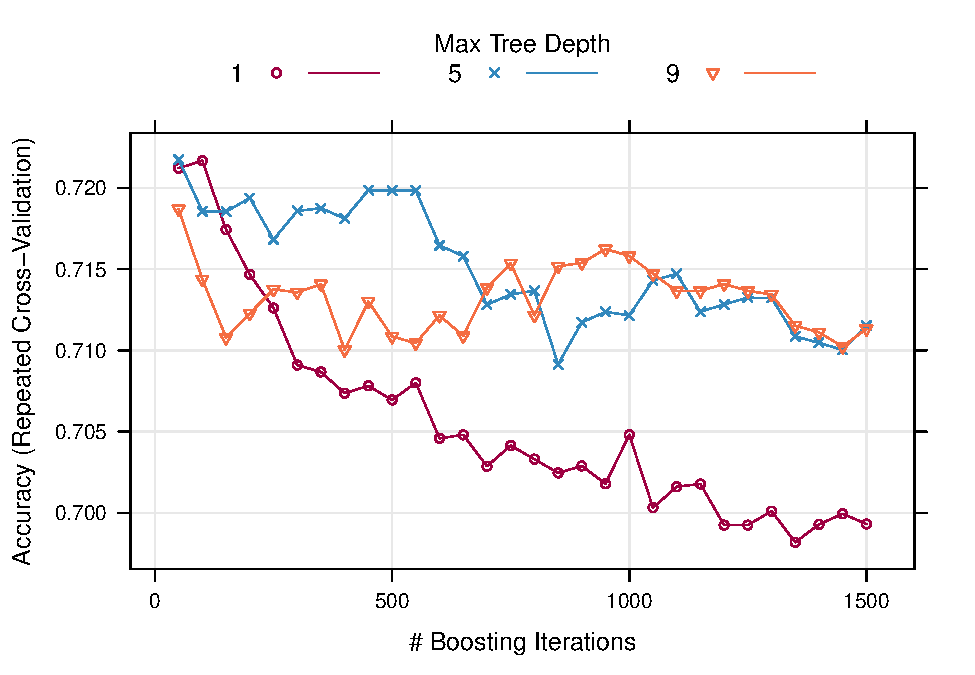
\includegraphics{article_files/figure-latex/plot_variable_importance-1.pdf}
%\end{figure}

\begin{figure}[htbp]
\centering
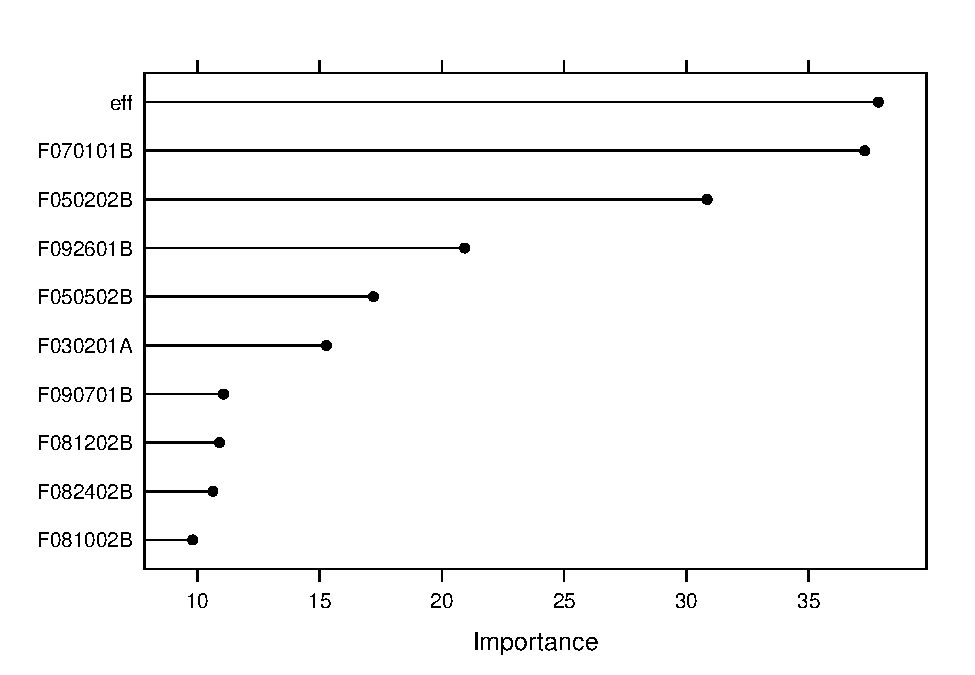
\includegraphics[width = 0.5\textwidth]{article_files/figure-latex/plot_variable_importance-2.pdf}
\caption{Importance of top 10 variables}\label{varimp}
\end{figure}


\begin{figure}[htbp]
\centering
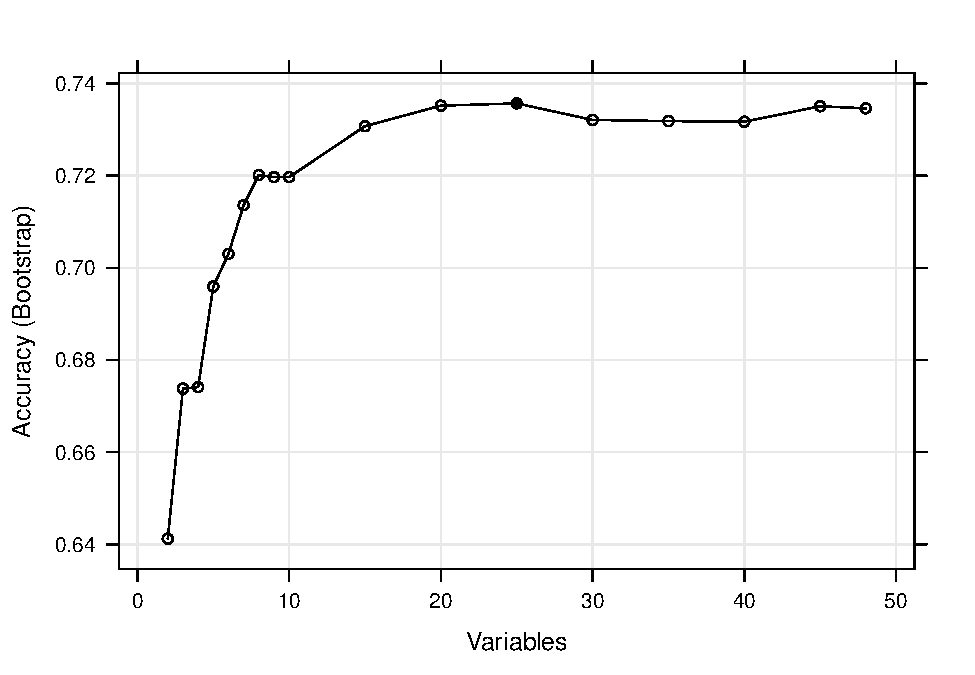
\includegraphics[width = 0.5\textwidth]{article_files/figure-latex/plot_feature_selection-1.pdf}
\caption{best number of variables for prediction}\label{feature_selection}
\end{figure}
It is shown that although the best number of  variables is 25 for the predition, however, the top 5 or 10 contribute most to the predition accuracy. for simplicity, we choose the top
5 most important variables, explore the difference of accuracy using
a variaty of machine learning methods.
Table 1 shows the results of predicting accuracy using different machine learning methods with and without the feature of DEA efficiency. The accuracy would be improved with the efficiency, with an increase ranging from 1\% to 6.5\%. In each of the machine learning method, a variety of parameters were tested to obtain the best performance. 
\begin{verbatim}
##      method Accuracy_without_eff Accuracy_with_eff
## 1 svmLinear            0.6357143         0.7071429
## 2        rf            0.6571429         0.6857143
## 3        nb            0.7142857         0.7428571
## 4      C5.0            0.7571429         0.7714286
## 5       gbm            0.7428571         0.7500000
## 6       glm            0.6857143         0.7071429
## 7  multinom            0.6857143         0.7071429
\end{verbatim}


\subsection{Conclusion}\label{conclusion}
To improve the prediction accuracy of business failure, The data from 2004-2010 was collected and examined. It was found that ST corporations had average lower efficiency than those Non-ST corporations. DEA efficiency was introduced and the results showed that efficiency did provide valuable information for better accuracy. Amoung the 7 prediction models, C5.0 had the best performance.



\subsection{Reference}\label{reference}

\bibliography{library.bib}
%\begin{enumerate}
%\def\labelenumi{\arabic{enumi}.}
%\item
%  Breiman, Leo (2001). ``Random Forests''. Machine Learning 45 (1):
%  5--32. \url{doi:10.1023/A:1010933404324}.
%\item
%\end{enumerate}

\end{document}
